% 建议使用 XeLaTeX 或 LuaLaTeX 编译(更佳的中文支持)
\documentclass[UTF8,zihao=-4]{ctexart}

% 统一导言
\usepackage[a4paper,margin=2.5cm]{geometry}
\usepackage{amsmath,amssymb,amsthm}
\usepackage{bm}
\usepackage{hyperref}
\usepackage{graphicx}
\usepackage{caption}
\usepackage{listings}
\usepackage{xcolor}
\usepackage{float}
\usepackage{placeins}

% 图片路径
\graphicspath{{figures/}}

% 统一代码风格
\lstdefinestyle{code}{%
  language=Python,
  basicstyle=\ttfamily\small,
  numbers=left,
  numberstyle=\tiny,
  keywordstyle=\color{blue}\bfseries,
  commentstyle=\color{teal!70!black},
  stringstyle=\color{orange!70!black},
  breaklines=true,
  frame=single,
  rulecolor=\color{black!30},
  tabsize=2,
  showstringspaces=false
}
\lstset{style=code}

\title{XGBoost:理论与实践}
\author{}
\date{\today}

\begin{document}
\maketitle

% 结构:Introduction / Theory and Formulas / Applications and Tips / Python Practice / Result / Summary

\section{引言}
XGBoost 是高效、可扩展的梯度提升树(GBDT)实现。它通过二阶近似优化、稀疏感知的分裂查找、学习率(shrinkage)与行/列子采样、以及显式结构正则化等机制,兼顾训练效率与泛化性能。

\section{原理与公式}
梯度提升以逐步加法模型 $F_M(\mathbf{x})=\sum_{m=1}^M f_m(\mathbf{x})$ 拟合弱学习器(浅树),XGBoost 最小化带正则的目标:
\begin{equation}
\mathcal{L} = \sum_{i=1}^n \ell\big(y_i, \hat{y}_i\big) + \sum_{m=1}^M \Omega(f_m), \quad \Omega(f)=\gamma T + \tfrac{1}{2}\lambda \lVert w \rVert^2,
\end{equation}
其中 $T$ 为叶子数、$w$ 为叶子打分。对损失在当前预测处做二阶泰勒展开,得到节点上梯度 $g_i$ 与海森 $h_i$ 的求和,左右子集 $L,R$ 的分裂增益为:
\begin{equation}
\mathrm{Gain} = \tfrac{1}{2}\! \left( \frac{\big(\sum_{i\in L} g_i\big)^2}{\sum_{i\in L} h_i + \lambda} + \frac{\big(\sum_{i\in R} g_i\big)^2}{\sum_{i\in R} h_i + \lambda} - \frac{\big(\sum_{i\in L\cup R} g_i\big)^2}{\sum_{i\in L\cup R} h_i + \lambda} \right) - \gamma.
\end{equation}
通过 $\lambda,\gamma$ 的结构正则、学习率(shrinkage)、列/行子采样、深度与叶子约束来控制模型复杂度与过拟合。

\section{应用与技巧}
\begin{itemize}
  \item \textbf{特征与缩放:} 支持数值与独热编码后的类别特征;树模型通常无需标准化。
  \item \textbf{关键超参:} \texttt{n\_estimators}、\texttt{max\_depth}、\texttt{learning\_rate}、\texttt{subsample}、\texttt{colsample\_bytree}、\texttt{reg\_alpha}/\texttt{reg\_lambda}。
  \item \textbf{早停:} 使用 \texttt{eval\_set} 与 \texttt{early\_stopping\_rounds} 在验证集上早停。
  \item \textbf{类不平衡:} 设置 \texttt{scale\_pos\_weight} 或采用分层采样。
  \item \textbf{解释性:} 内置重要性可作初筛;更稳健可用置换重要性或 SHAP。
\end{itemize}

\section{Python 实战}
在本章节目录运行下述命令,图片将保存到 \texttt{figures/}:
\begin{lstlisting}[style=code,caption={生成 XGBoost 配图},label={lst:genfigs_xgb_cn}]
python gen_xgboost_figures.py
\end{lstlisting}

% 纳入完整 Python 源码
\lstinputlisting[style=code,caption={gen\_xgboost\_figures.py 源码},label={lst:source_xgb_cn}]{gen_xgboost_figures.py}

\section{结果}
\begin{figure}[H]
  \centering
  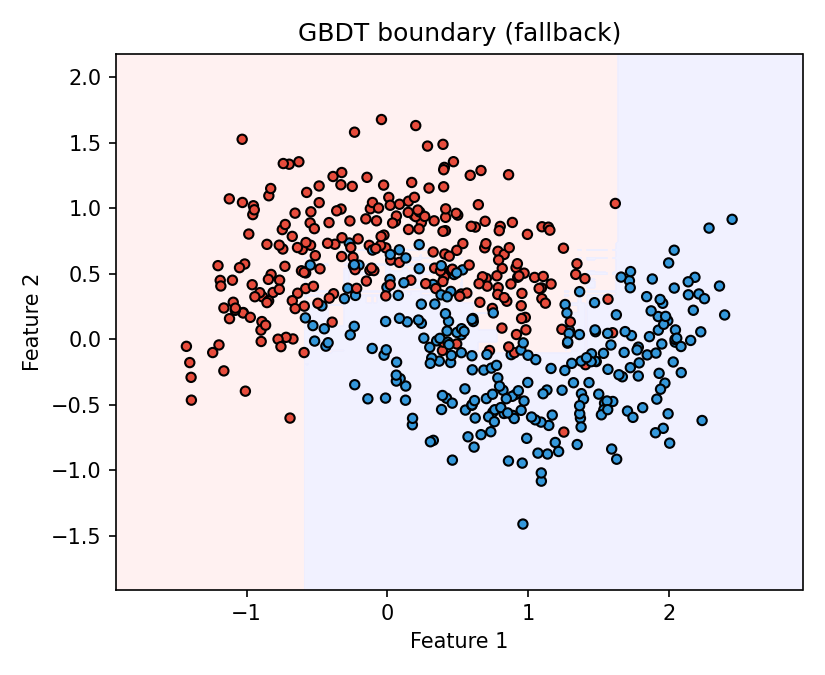
\includegraphics[width=0.9\linewidth]{xgb_decision_boundary_2class.png}
  \caption{XGBoost 在两类数据上的决策边界。}
  \label{fig:xgb2_cn}
\end{figure}
\FloatBarrier

\begin{figure}[H]
  \centering
  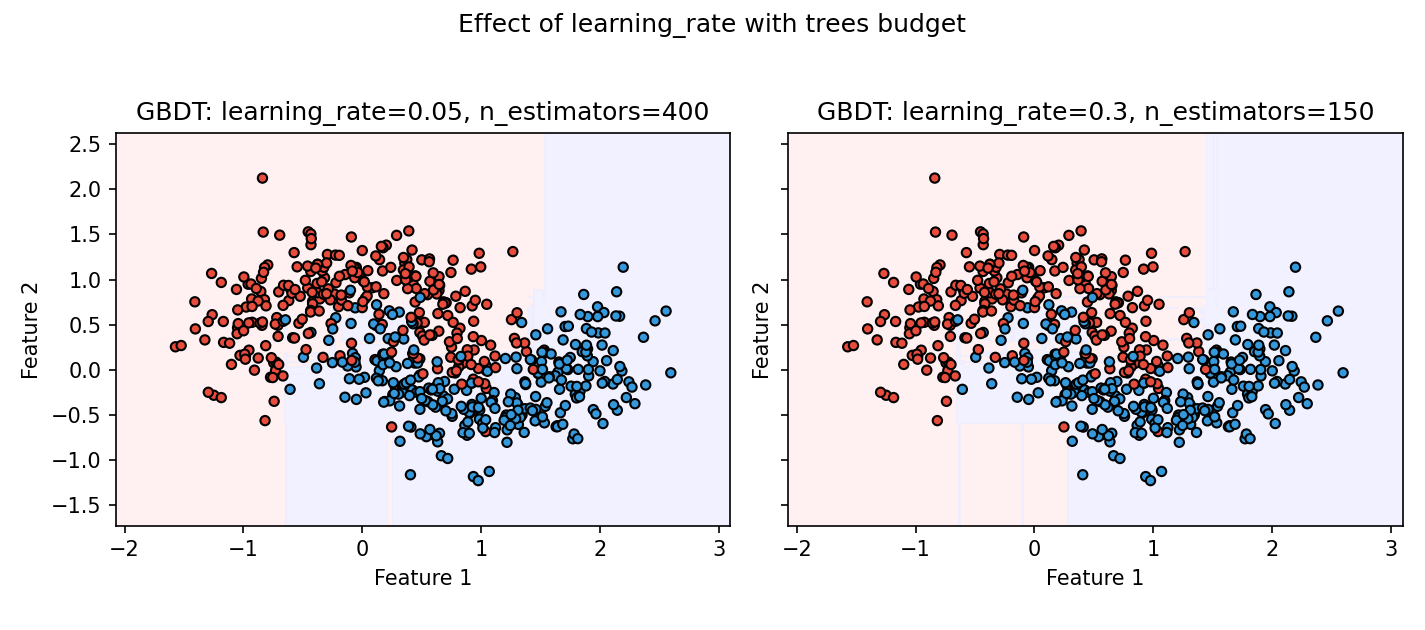
\includegraphics[width=0.95\linewidth]{xgb_learning_rate_compare.png}
  \caption{在固定树预算下,不同学习率的效果对比。}
  \label{fig:xgb_lr_cn}
\end{figure}
\FloatBarrier

\begin{figure}[H]
  \centering
  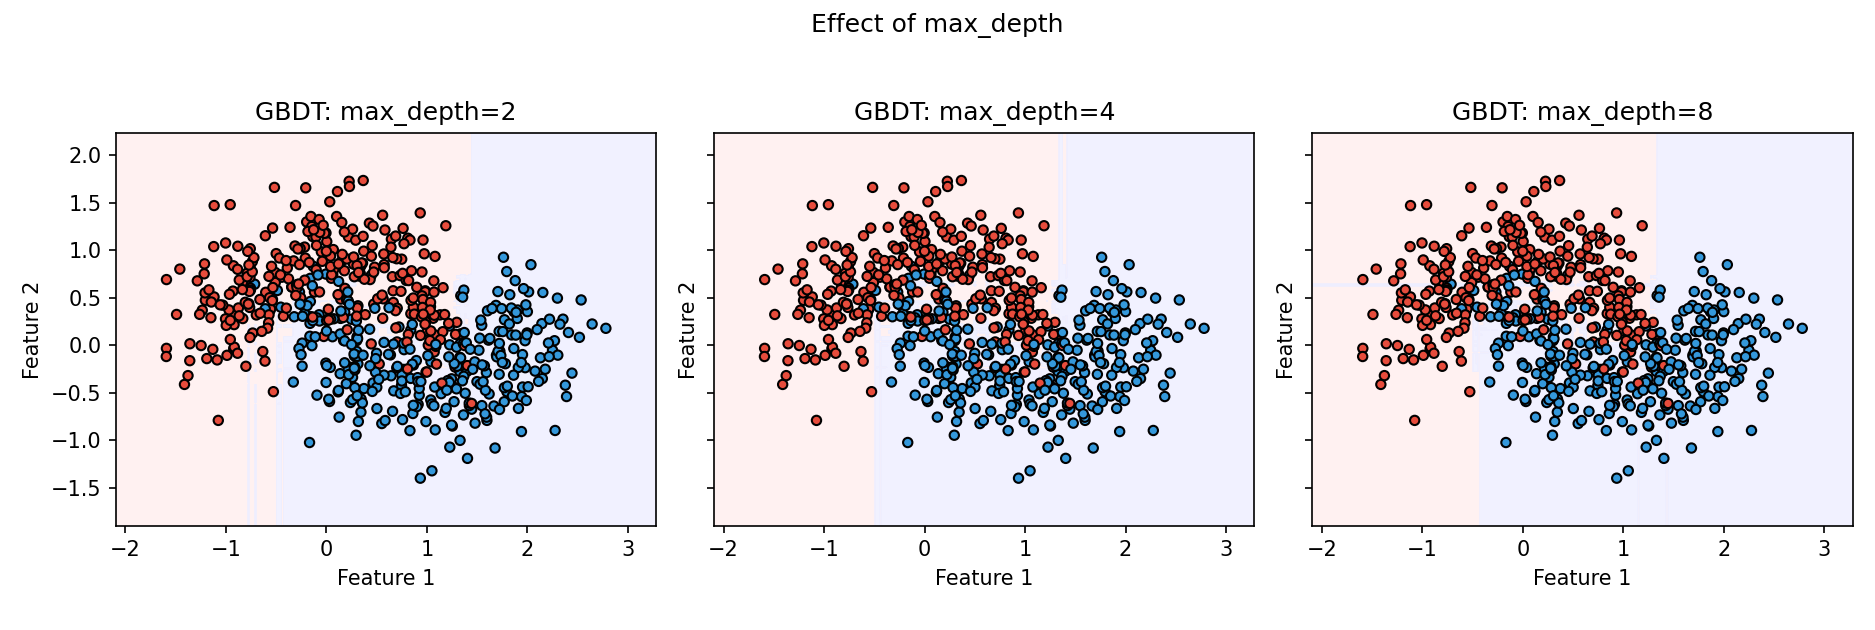
\includegraphics[width=0.95\linewidth]{xgb_max_depth_compare.png}
  \caption{不同 \texttt{max\_depth} 下的决策边界对比。}
  \label{fig:xgb_depth_cn}
\end{figure}
\FloatBarrier

\begin{figure}[H]
  \centering
  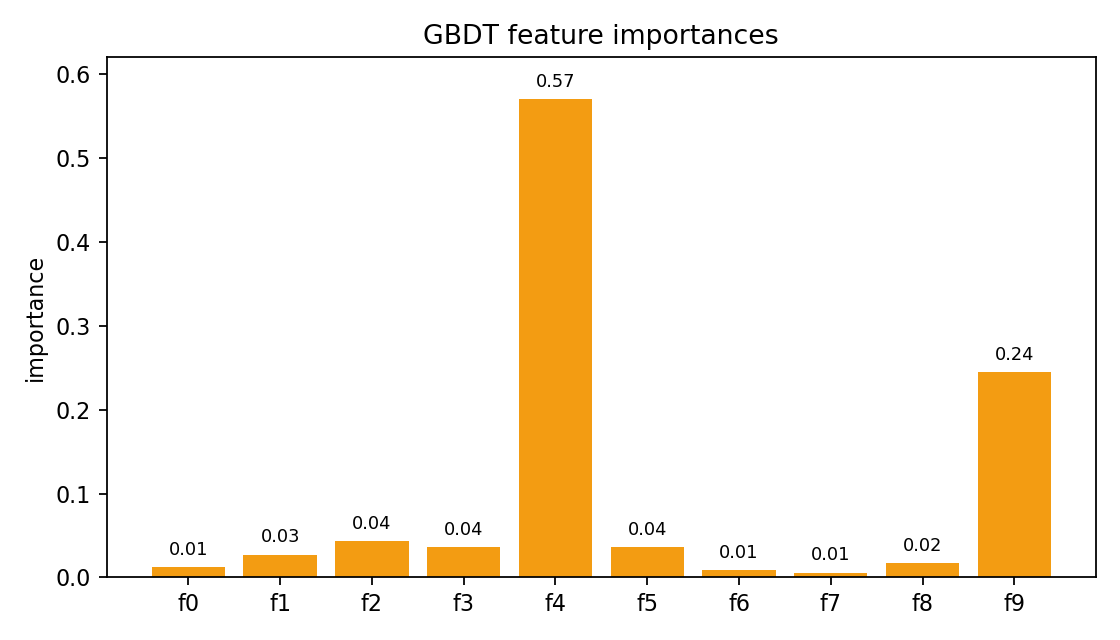
\includegraphics[width=0.85\linewidth]{xgb_feature_importances.png}
  \caption{XGBoost 的特征重要性。}
  \label{fig:xgb_fi_cn}
\end{figure}
\FloatBarrier

\begin{figure}[H]
  \centering
  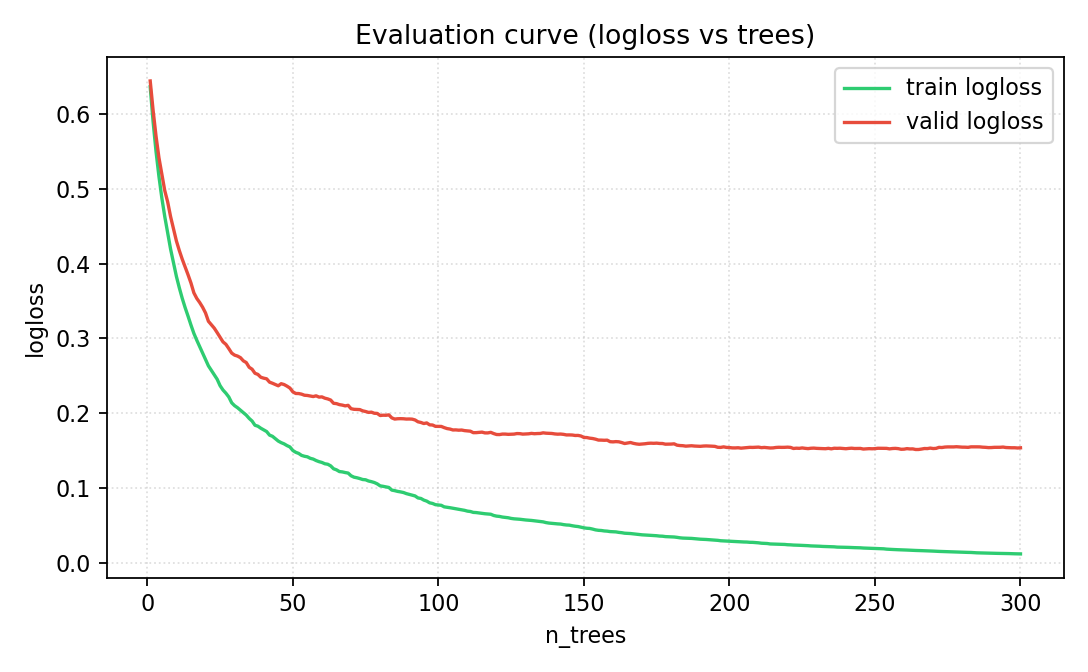
\includegraphics[width=0.85\linewidth]{xgb_eval_logloss_curve.png}
  \caption{训练/验证 logloss 随树数变化的曲线。}
  \label{fig:xgb_eval_cn}
\end{figure}
\FloatBarrier

\section{总结}
XGBoost 在高效的树提升框架上引入结构正则、二阶近似与稀疏感知的分裂查找,并结合学习率与采样策略,在表格数据任务中具有很强的基准表现。通过调节深度、学习率与采样比例,可在偏差-方差与计算开销之间取得良好平衡。

\end{document}

